\documentclass[conference]{IEEEtran}
% generated by Docutils <http://docutils.sourceforge.net/>
\usepackage{fixltx2e} % LaTeX patches, \textsubscript
\usepackage{cmap} % fix search and cut-and-paste in Acrobat
\usepackage{ifthen}
\usepackage[T1]{fontenc}
\usepackage[utf8]{inputenc}
\usepackage{float} % float configuration
\floatplacement{figure}{H} % place figures here definitely
\usepackage{graphicx}
\usepackage{multirow}
\usepackage{longtable,ltcaption,array}
\setlength{\extrarowheight}{2pt}
\newlength{\DUtablewidth} % internal use in tables

%%% Custom LaTeX preamble
% PDF Standard Fonts
\usepackage{mathptmx} % Times
\usepackage[scaled=.90]{helvet}
\usepackage{courier}

%%% User specified packages and stylesheets

%%% Fallback definitions for Docutils-specific commands

% hyperlinks:
\ifthenelse{\isundefined{\hypersetup}}{
  \usepackage[colorlinks=true,linkcolor=blue,urlcolor=blue]{hyperref}
  \urlstyle{same} % normal text font (alternatives: tt, rm, sf)
}{}
\hypersetup{
  pdftitle={A comparison of networked game development APIs},
}

%%% Title Data
\title{\phantomsection%
  A comparison of networked game development APIs%
  \label{a-comparison-of-networked-game-development-apis}}
\author{}
\date{}

%%% Body
\begin{document}
\maketitle
\begin{abstract}
Networked game programming is complex compared to single
player games. Several libraries and platforms exist to ease the
development. In this exploratory study, we propose a technique for
evaluating how much a networked game development platform succeeds
in hiding complexity. We apply Sneed's Object-Points (OP) analysis
to two pre-existing implementations of the same minimal networked
multiplayer game: Pong. The OP technique succesfully illustrates
the different amounts of complexity the developer has to manage on
the two alternative platforms. We have automated the source-code
based analysis process, and suggest using it both for longitudal
studies of API development and for comparing alternative API
approaches.
\end{abstract}


\section{Introduction%
  \label{introduction}%
}

Networked application programming is generally more complex than
standalone software development. The developer typically needs to deal
with events, conflicts and error conditions originating from other
parts of the distributed system as well as the local user. This is
emphasized in multiuser real-time systems compared to the relatively
leisurely request-response interaction patterns of most client-server
applications. Developing a massively multiplayer online game (MMOG)
has been stated to typically take two to three times as long as
creating and launching a single-player game \cite{middleware}.

Higher level abstractions in software are a common way to attempt to
ease application development. Regarding networking, libraries exist to
simplify managing connections and messaging. On a even higher level,
distributed object systems automate remote calls and data
synchronization. For an application developer, these systems are
provided as a set of abstractions forming the application development
interface (API).

It has been noted how making good APIs is hard -{}- and that creating a
bad one is easy \cite{api-matters}. Even a small quirk in an API can
accumulate to substantial problems in larger bodies of application
code. API design has a significant impact on software quality, and
increased API complexity is associated with increased software failure
rate \cite{cmu-api_failures}.

An entity system for networked application development has been put
forth in {[}Alatalo2011{]}. Developed in the open source Tundra SDK, it
strives to apply best practices from game engine design literature,
notably the aggregation using entity-component model. Specifically for
networking, it features attribute autosynchronization, a simple form
of transparent remote procedure calls (entity actions) and efficient
customized movement messages with inter- and extrapolation logic (dead
reckoning). The purpose of the abstract entity model, and the whole
concrete platform, is to make multiplayer game development easy and
productive. The goal in this study is to evaluate whether and how the
Tundra API, and with it a a few common practices in modern game and
networking libraries, succeed in that.

How can a conceptual design of an entity system be really evaluated?
How can we know how well a platform supports actual networked game
development? These are not easy questions, but the answers would
really help us concretely in game and platform development. One
presentation of a MMOG middleware proposes four essential ``ease of''
requirements: ease of development, deployment, maintenance and
change. However in the evaluation they note the difficulty of
quantitative measurement of e.g. ease of development or change, and
review platform scalability only \cite{middleware}. Here we focus on the
difficult ease-of question instead. We do not claim to provide final
answers to all of it here. The area of software and API complexity
analysis has however made interesting progress recently
\cite{api-complexity-analysis,cmu-api_failures}. By applying a software
complexity analysis technique, we investigate one particular aspect of
the quality of networked application platforms: the API complexity for
a networked game developer.

We analyze API complexity by following an approach from a previous
study in a slightly different field \cite{api-complexity-analysis}. We
conduct a comparative study of two alternative APIs for networked game
development by analyzing the complexity of the same game implemented
on the two platforms. The game is Pong, which is proposed as a minimal
hello-world style example of a multiplayer game.

The article is organized as follows: Next, we provide background
information on API complexity research, the selected game case and the
alternative networked game development platforms. Then the conducting
and the results of the Object-Points analysis is presented. Finally,
results are discussed both to evaluate the applicability of the
analysis method, and in light of explaining factors from the APIs.

% (the point about leakages only in discussion? or somehow here too
% still? was:) The purpose is to identify leakage points in the
% abstractions in that entity system and propose areas for
% improvement.


\section{Background%
  \label{background}%
}


\subsection{The research methodology - of API complexity research%
  \label{the-research-methodology-of-api-complexity-research}%
}

Recently, software complexity analysis techniques have been applied to
statistical (quantitative) studies of API
complexity. \cite{cmu-api_failures} studies 2 large corporate software
projects and 9 open source projects and finds a link between API
complexity and increases in failure proneness of the software (bug
reports from the field). The masses of source code are quantified with
measures such as API size and dispersion. Building on existing work,
API complexity is calculated simply from the number of public methods
and attributes. In the discussion it is noted how this is severely
limited: for example, it fails to take into account pre- and
post-invocation assumptions of the API and possibly required sequences
of invocation \cite{cmu-api_failures}.

More generally, API usability research has recently gotten attention
in human centric research. Both traditional HCI usability evaluation
techniques have been adapted to API evaluation, and also novel
approaches specific to API usability research have been put forth
\cite{conceptmaps}. Traditional techniques include the think aloud
protocol, heuristic evaluation and cognitive walkthoughs
\cite{overview}. Metrics in those studies include for example the
completion times of predefined tasks. Human observation based API
evaluation is challenging due to several reasons, compared to
usability studies of simpler tasks accomplished with GUIs. Developing
even a small application takes easily weeks so it is difficult to fit
valid tasks in a typical 1-2 hour observation session
\cite{conceptmaps}.

Novel approaches developed especially for API evaluation and
development include peer reviews \cite{apipeerreview}, walkthroughs and
the concept maps method \cite{conceptmaps,overview}. These avoid the
problems of traditional HCI methods, notably by involving real world
usage of the API over a long period of time. They are still
considerably laborsome and essentially qualitative analysis. We plan
to conduct such studies in future work on network game platform
development.

Here, however, we investigate the suitability of quantitative and even
automated API complexity measures. We base the analysis on existing
bodies of source code, which has several advantages: real world data
(source codes of existing applications) can be applied, and the
analysis can be quick being not very laborsome and giving immediate
feedback. Longitudinal studies of API development over time can be
straightforward to conduct by running the analysis for different
versions of the software. If fully automated, the analysis can be even
run as a part of a continuous integration setup.

To address the issue of too simplistic software metrics (such as lines
of code count), we apply the relatively sophisticated Object-Points
(OP) analysis by Sneed. It has been proposed for API complexity
evaluation in \cite{api-complexity-analysis}, where four alternative
implementations, on different frameworks, are used for a comparative
analysis. OP has originally been developed for estimating development
effort, but there the authors adopt it to calculate the complexity of
existing software for complexity comparisons. Number of classes, their
members and the set of operations called are counted and assigned
adjustment weights in the calculation. A key decision is to apply a
surrogate measurement: the APIs are not analyzed directly, but
programs developed against them are analyzed. The focus is on how a
API is used, which is in line with the practice in the aforementioned
HCI studies. Measuring the complexity, for example the sizes, of the
APIs themselves would give misleading results, as a more complete API
would appear more complex, even if it provided good concepts so that
the task at hand could be in fact accomplished with just a small
subset of the full API. In OP analysis, intermediate UML models are
used as the data source which allows comparing programs in different
languages \cite{api-complexity-analysis}. Importantly, the Sneed measure
allows direct tracking from indicator values to program
structures. This is elemental for the purposes of API evaluation and
design -{}- for example if many codebases get a high proportion of their
complexity value due to a specific part of the API, it can then be
examined qualitatively.


\subsection{The game of Pong%
  \label{the-game-of-pong}%
}

We propose using Pong as a minimal networked multiplayer game. It is
tiny in functionality, but still demonstrates key issues with
networking and games with the combination of the clients controlling
their own paddles and the ball bouncing in the shared space. Pong has
been used in networked game research earlier, recently in an
interesting study of latency compensation techniques
\cite{pong-ping}. Also even a minimal game suffices to reveal the amount
of software needed for all the basics: establishing connections,
handling players joining in and dropping out, and just getting the
networked software up and running.

For further studies, devising a set of different kind of small games,
and perhaps some larger sufficiently complex game, would really allow
rich comparative API analysis.


\subsection{Platforms: realXtend Tundra SDK and Union Platform%
  \label{platforms-realxtend-tundra-sdk-and-union-platform}%
}

For this initial study, we selected two relatively high-level
networked game platforms: realXtend Tundra SDK (open source) and the
Union Platform (closed source proprietary). They bear several key
similarities and differences which are interesting for the study:

Both Tundra and Union are specifically for networking, and expose it
to the developer on an abstract application level. That is, the games
do not know anything about sockets or network hosts. Instead, an
abstract container object is provided (Room in Union, Scene in
Tundra). Application logic listens to events from the container, for
example when a new client joins the shared session/space.

Also, both platforms provide an automated mechanism for synchronizing
state over the network. The shared state is in special attributes
(objects of type Attribute), which are in the container (in Union
directly in the Room object, in Tundra in entities in the Scene). The
attributes are automatically shared among all the participants, and
provide events for interested parties to get notified of changes. This
way it is simple to for example set the game score points on the
server, and show it in the GUI in clients.

However, there is one fundamental difference in the platforms and how
they are used in the Pong examples studied here. TundraPong is a
script running on the Tundra platform. UnionPong is a new client
application, to which the networking has been added by using Union's
Reaktor Flash library. The Tundra game utilizes a complete static
scene datafile where the game logic just starts moving objects
around. It runs on an existing client-server system, and utilizes
several default components from the platform: notably all the data for
the appearance and spatial instancing. In contrast, UnionPong not only
has code to create the appearance of the game court (as it is called
in Court.as), but also to define what data is required for a spatial
moving object (PongObject has x, y, direction, speed, width and
height). Tundra, again, has the position in the builtin predefined
Placeable component and the size and shape information for collisions,
and the speed vector for movement, in the physics module's Rigidbody
component. Also with networking there is a great difference: OnionPong
sends own custom movement messages for all the movement, and has also
custom server side code to do ball bouncing, whereas on Tundra the
default movement replication and physics collisions are used.

So it is clear at the start that UnionPong is more complex, due to
having much more of the implementation in the game/application
code. The analysis is still interesting as it helps to answer the
questions at hand: a) how much do the alternative APIs manage to hide
complexity and b) how well does the selected analysis technique apply
to networked game API evaluation.

For more results, at least these two additional Pong implementations
should be added to the analysis in future work:

1. An alternative TundraPong style game where the defaults from an
underlying platform are used to the fullest, for example with the
Unreal engine.

2. A version made with a different networked programming paradigm,
such as the Emerson language which is a Javascript variant by the
Sirikata project for networked applications, without attribute
autosynchronization but using messaging exclusively instead
\cite{sirikata-scripting}.

The analysis here is limited to the two platforms simply because we do
not have more implementations (Pong source codes) to study yet. Also
we find that a careful review is in place first to evaluate the
suitability of this kind of Object-Points analysis, before continuing
to apply it more. The Tundra one was initiated by the author (only the
scene and trivial computer opponent logic as a test), and later
completed by an independent developer (he made all the networking and
game control code). The Union one we found with an Internet search.


\section{Application of Object-Point analysis%
  \label{application-of-object-point-analysis}%
}

The chosen Sneed's Object-Point (OP) analysis was conducted by
automating the collection of most of the key data to derive the
variables in the equation. We apply the technique following what has
been used for API complexity analysis before in
\cite{api-complexity-analysis}. Here we give a brief overview of Sneed's
OP analysis itself, and describe how we derive the data from source
code analysis.


\subsection{Sneed's Object-Point analysis%
  \label{sneed-s-object-point-analysis}%
}

(NOTE: this is a little a new background treatment again - consider
moving some of this to 2. etc XXX)

Software cost estimation has been of paramount importance in the field
of software engineering, and various approaches have been developed
for it through the decades. The early COCOMO model uses simply program
size (lines of code) to estimate development effort, but later the
Function-Point, Data-Point and finally Object-Point methods base the
analysis on functionality and other properties of the program
\cite{henrich97repositorybased}. Recently the Object-Point (OP) method has been
used for analysing existing implementations, for API complexity
comparison purposes, even though it was originally developed for early
work estimate analysis based on UML design diagrams
\cite{api-complexity-analysis}. Arguably, it is rich enough to explore
structural and dynamic properties of software for meaningful
complexity data.

For example in the preceeding API complexity analysis OP study that we
follow here, two of the four compared implementations would get the
opposite results in a simplistic lines of code (LOC) analysis. That
is, the PHP implementation there features only 48 LOC but results in
356.34 OP, whereas the domain specific language (DSL) version is 144
LOC and 266.76 OP \cite{api-complexity-analysis}. Their explanation is
that ``an API user is only exposed to an API feature chunk of low
structural complexity'', as the chunk's ``size is limited in terms of
participating classes and the smallest number of operations per class''
and it ``shows a relatively weak connectedness of classes (H = 1),
resulting from the small number of associations and generalizations
between the classes''.

That is of utmost importance to our interest in making networked game
development easier with a good API. We are after a limited set of good
concepts with clear interactions that a game developer could learn
easily and grow to master. Not all lines of code are equal -{}- a bad
API makes it a struggle to get even a few operations working if the
developer has to hunt for functionality that is scattered around in an
incoherent way.

The Object-Points, as applied here, are a sum of two parts: Class
Points (CP) and Message Points (MP).

% "While the original definition of the OP measure [17] involves a
% third sum- mand for expressing the Use Case (UC) complexity (e.g.,
% based on a UML use case model of the underlying application
% scenario), we can omit this summand in our experiment. This is
% because in our comparative experiment based on a single application
% scenario, we take the UC complexity as a constant."

\textbf{Class points, CP} is calculated from the static class structure,
specifically: the class count and sums of attribute, operation and
relation counts. Weights are used to correct the values for the
overall calculation. Class inheritance is taken into account by
calculating novelty weights for specializing classes.

\textbf{Message points, MP} is defined by the set of operations
(functions/methods) \emph{actually used} in the software. First, the number
of operations is used. Then the parameter count for each called
operation is collected. Also the source and target counts of the
operation calls are established. Again, novelty weights are used to
compensate for repeated occurrences due to subclassing.

TODO: add the equation + legend here -{}- but refer to the other paper
for more, or do we need to explain every detail here too?


\subsection{Reading class and interaction data from source code%
  \label{reading-class-and-interaction-data-from-source-code}%
}

To read the \emph{static class data} for the \textbf{Class Points} (CP), we
utilize existing source code parsing and annotation systems in API
documentation tools. The first alternative implementations of a
minimal networked game on different modern high-level APIs studied
here are written as a a) Javascript application and b) a combination
of Actionscript (as3) for the client and Java for the server
module. We developed parsers for the internal / intermediate
representation of class and method signatures of JsDoc JSON and
AsDoc XML. (The single Java class for b) server we may analyze
manually). The class information is read in a Python application to an
internal model which contains the data for the Sneed points
calculation, implemented in another module in the same Python
application.

For the \emph{dynamic function call} information, to calculate the
\textbf{Message Points} (MP) in the overall OP analysis, we use the Closure
Javascript compiler to traverse the source code to collect function
calls and their argument counts. To be able to analyze also
Actionscript code, we do text processing to strip AS extensions to the
basic ECMA/Javascript (remove public/private definitions and type
declarations). A parser made with Python is used to read the function
call data required to calculate MPs. This completes the automated data
collection and processing developed for the OP calculations here.

Finally, to facilitate manual validation and visual communication of
the data mined from the source codes, we added functionality to create
UML class diagrams from the very same in-memory data structure which
is used for the OP calculation. We chose the UXF format of the open
source Umlet GUI diagram tool, due to it's simple and straightforward
XML document format and the even simpler plaintext syntax used to
describe the individual UML elements, such as a class or a
relation. It is useful to be able to manually edit the diagrams
further with the GUI tool to improve the layout and add notes.

All this software to run the calculations, together with the datasets
used in the analysis here, is available from
\url{https://github.com/realXtend/doc/tree/master/netgames/tools/}
(pointcounter.py is the executable, with the implementation of the
equation).

Repository based automatic queries for OP analysis have been presented
earlier in \cite{henrich97repositorybased}. There a repository of
\emph{documents}, or abstract software design models (PCTE) is queried for
automatic OP calculations using the P-OQL language. We are not aware
of previous implementations of deriving data for OP calculations from
source code only. Automating the calculation opens up fascinating
possibilities for platform and API development in future work, such as
longitudal evaluation of API complexity evolution, and dissecting a
body of software by running a series of calculations to pinpoint
potential sources of complexity.


\section{Results%
  \label{results}%
}

The results for the Object Points analysis for the two codebases are
presented in table 1.

\setlength{\DUtablewidth}{\linewidth}
\begin{longtable*}[c]{|p{0.145\DUtablewidth}|p{0.179\DUtablewidth}|p{0.075\DUtablewidth}|p{0.121\DUtablewidth}|}
\hline
\multirow{2}{0.14\DUtablewidth}{%\textbf{%
(measure)
}} & \multirow{2}{0.18\DUtablewidth}{%\textbf{%
TundraPong
(client and
server)
}} & \multicolumn{2}{p{0.20\DUtablewidth}|}{\textbf{%
UnionPong
Client
}} \\
\cline{3-3}
\cline{4-4}
 &  & \textbf{%
Full
} & \textbf{%
Net
} \\
\hline
\endfirsthead
\hline
\multirow{2}{0.14\DUtablewidth}{%\textbf{%
(measure)
}} & \multirow{2}{0.18\DUtablewidth}{%\textbf{%
TundraPong
(client and
server)
}} & \multicolumn{2}{p{0.20\DUtablewidth}|}{\textbf{%
UnionPong
Client
}} \\
\cline{3-3}
\cline{4-4}
 &  & \textbf{%
Full
} & \textbf{%
Net
} \\
\hline
\endhead
\multicolumn{4}{c}{\hfill ... continued on next page} \\
\endfoot
\endlastfoot

Lines of
Code
 & 
361
 & 
565
 & 
420
 \\
\hline

Number of
classes
 & 
2
 & 
14
 & 
8
 \\
\hline

Class
Points
 & 
75
 & 
180
 & 
140
 \\
\hline

Message
Points
 & 
68
 & 
136
 & 
124
 \\
\hline

Object
Points
 & 
143
 & 
316
 & 
264
 \\
\hline
\end{longtable*}

% 20 4 51 1
% OP 178 = CP 75 + MP 103
% 
% ..
% 
% ..
% 
% without params in MP calc:
% 
% 67 22 135 0.807692307692
% OP 316 = CP 180 + MP 136
% 
% 44 20 96 0.875
% OP 264 = CP 140 + MP 124

For TundraPong, the single Javascript source file (assets/game.js) is
included. It features both client and server functionality in two
classes respectively. It is the complete implementation with GUI and
the minimal game session management.

For UnionPong, all the client side ActionScript files (14) are
included for the full run, and selected 8 for the network code only
calculation. The selection is made on the class level: the classes
which involve networking are included in full, not edited line-by-line
to include networking code only. The included classes are:
GameManager, GameStates, KeyboardController, PongClient, PongObject,
RoomAttributes, RoomMessages, UnionPong. The excluded classes cover
GUI, the 2d scene implementation and general settings and utilities,
and are called: clamp, ClientAttributes, Court, HUD, Rectable and
Settings.
%
\begin{itemize}

\item UnionPong/Java/PongRoomModule.java

\end{itemize}


\subsection{Only the networking code%
  \label{only-the-networking-code}%
}

NOTES:
%
\begin{itemize}

\item Selected classes, explain the criteria.

\end{itemize}

Class level selection - all classes which are involved in networking

KeyboardController is included because it is exactly what sends the
remote control messages from the player to the server (modifies
client.paddle's attributes and says client.commit()).

client 8x .as: 147.0

A better take: select only code for which there is a corresponding
part in the Tundra impl? Would leave the networking API, right? Well,
with a quick read through all of the code at least, the class based
selection did that -{}- the remaining classes are mostly network code /
code involving networking.


\subsection{UML Diagrams%
  \label{uml-diagrams}%
}

The data used in the calculations is also generated to UML class
diagrams by the analysis software, for manual verification of the
source code analysis process, and for (XXX thinking about the
codebases \& complexity calcs).
\begin{figure}
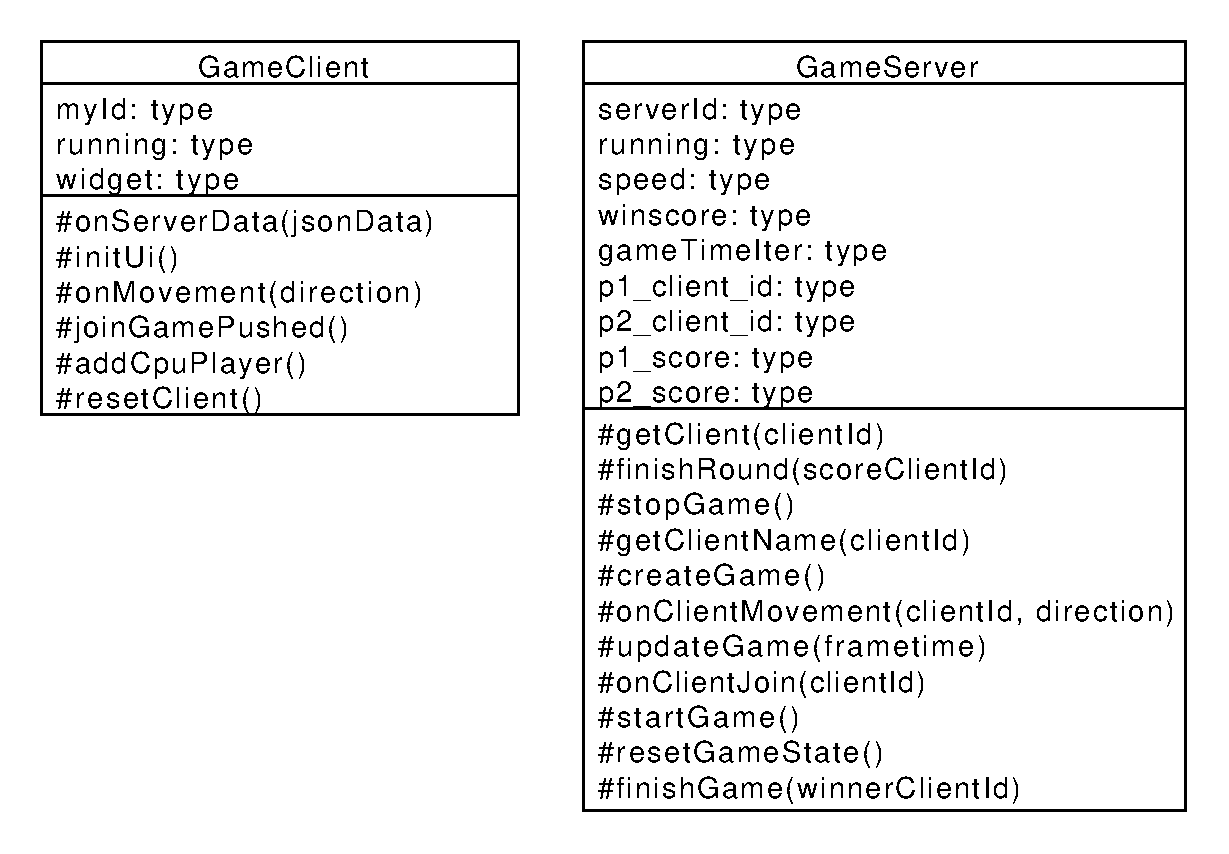
\includegraphics[scale=0.400000]{pics/TundraPong.pdf}
\caption{The two classes in TundraPong game.js.}
\end{figure}
\begin{figure}
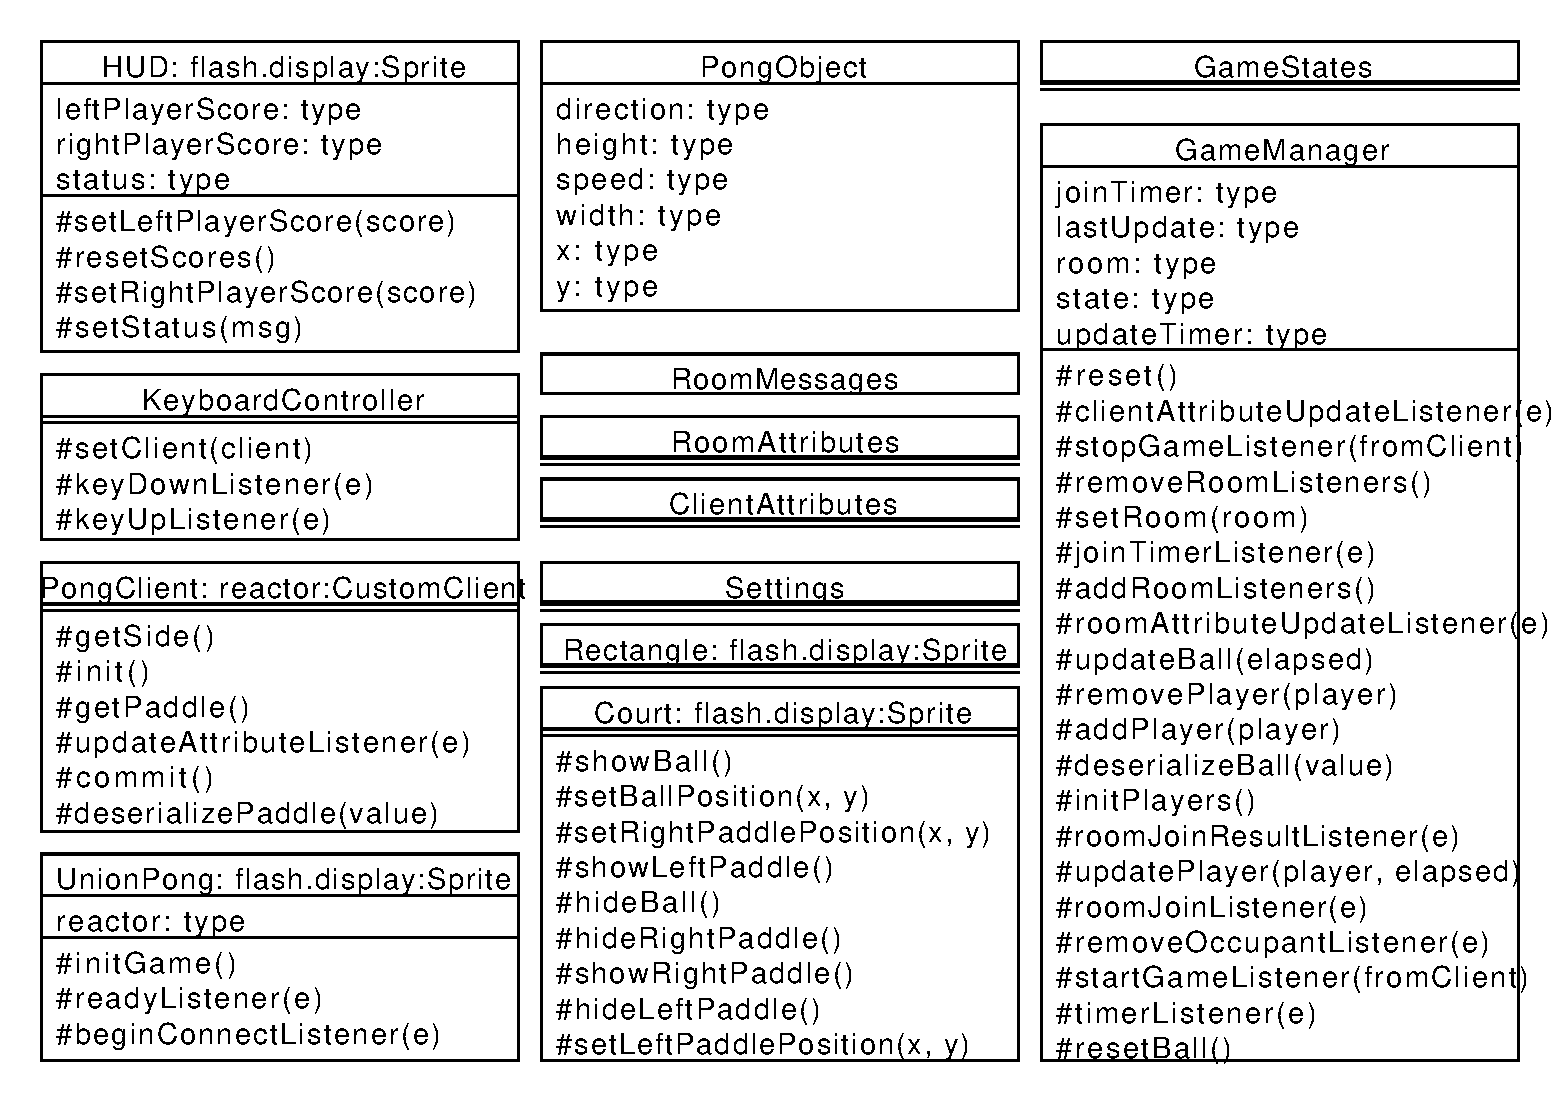
\includegraphics[scale=0.350000]{pics/UnionPong-manuallayout.pdf}
\caption{The 13 classes in UnionPong client side ActionScript.}
\end{figure}


\section{Discussion%
  \label{discussion}%
}

How should we interpret this result? There are several things to
consider, these are visited in the following: A. validity of the
analysis technique, the automated (partial) Object-Point
analysis B. nature, suitability and use of scripting vs. application
development libraries C. observations of the high-level network
programming APIs studied here. D. limitations: the many areas of
analysis outside the focus here (scalability, efficiency of the
networking etc)


\subsection{Validity of the analysis%
  \label{validity-of-the-analysis}%
}

We apply Sneed's Object-Point analysis, following how it has been
adopted to API complexity evaluation in \cite{api-complexity-analysis}, as
closely as we could with the automated source code analysis. The
validity must thus be evaluated from two viewpoints: a) applicability
of OPs to API complexity analysis in general and b) the deviations
from the intended calculation due to limits of the analysis software.

The OP sums of the full examples have an order of magnitude
(right? XXX) sized difference in the proposed complexity of the two
implementations of the same game. Noting the aforementioned
substantial difference in the nature and scope of the implementations,
the ratio of 74:273 (XXX fix when nums update) seems correct for
codebases of 2 sizeable and 14(+1) mostly small classes respectively.

TODO: what was left out from analysis (was anything, in the end? XXX)


\subsection{On scripting vs own client development%
  \label{on-scripting-vs-own-client-development}%
}

TODO - noting: higher points does not mean that Union is bad, but
highlights the difference of what Tundra and Union are -{}- right?
%
\begin{itemize}

\item as the data points out, implementing something on an existing
platform can be comparatively very little work

\item making an own application (client) is easily powerful and
straightforward for own custom things, however

\item same existing modules/components can be used either way,
though. still simpler when don't need to deal with application init
and connecting etc.

\item does the complexity lurk somewhere still?

\end{itemize}


\subsection{Observations of the high-level network programming APIs%
  \label{observations-of-the-high-level-network-programming-apis}%
}

The APIs under study here are very similar regarding the
networking. They both have an abstract container for the state: a Room
in Union, and a Scene in Tundra. Application can put own custom state
information as special attributes in that container, and the system
takes care of automatically synchronizing changes to that data.

Both use callbacks heavily, for example both to listen to new clients
entering the service (an event of Room in Union's Reaktor and in the
RoomModule on the Union server separately, an event of the Server core
API object in Tundra on server side) and to attribute changes coming
in over the network.

They both also allow sending simple ad-hoc custom messages, which the
Tundra version uses for game events such as informing of a victory
(with the associated data), and UnionPong uses for all networking
(also paddle and ball movements).

With this in mind, we would expect the difference in the complexity
sum derive from the scope of the implementations used in the analysis.

TODO: return to this when the numbers from network-code-only analysis are in too?!?


\subsection{Limitations%
  \label{limitations}%
}

the many areas of analysis outside the focus here (scalability,
efficiency of the networking, security, ..)

The minimal examples may not be complete, true networked play
implementations with error checking etc. (can we check this?)

TODO


\section{Conclusions%
  \label{conclusions}%
}

TODO

(We are happy and curious about using this tool for many kinds of
comparisons: longitudal studies of a single API over time, comparisons
of e.g. networking stacks when using different protocols for similar
functionality, ... or?)

Similarities and differences of using a platform as ready made client
software, on which just run scripts, vs. libraries to create own
applications, are interesting to study more. Same software components
(libraries, modules etc) can be used in both configurations -{}- what is
more suitable may well depend on the particular case.

(XXX Q: where does complexity lurk? should we consider the leaks here?
does Onion have something to handle them? at least had the Attribute
setting exception in the java server XXX)

\begin{thebibliography}{henrich97repositorybased}
\bibitem[api-matters]{api-matters}{
Michi Henning, API Design Matters, Communications of the ACM Vol. 52 No. 5 \url{http://cacm.acm.org/magazines/2009/5/24646-api-design-matters/fulltext}
}
\bibitem[cmu-api\_failures]{cmu-api_failures}{
Marcelo Cataldo1, Cleidson R.B. de Souza2 (2011). The Impact of API Complexity on Failures: An Empirical Analysis of Proprietary and Open Source Software Systems. \url{http://reports-archive.adm.cs.cmu.edu/anon/isr2011/CMU-ISR-11-106.pdf}
}
\bibitem[api-complexity-analysis]{api-complexity-analysis}{
Comparing Complexity of API Designs: An Exploratory Experiment on DSL-based Framework Integration. \url{http://www.sba-research.org/wp-content/uploads/publications/gpce11.pdf}
}
\bibitem[pong-ping]{pong-ping}{
High and Low Ping and the Game of Pong. \url{http://www.cs.umu.se/~greger/pong.pdf}
}
\bibitem[sirikata-scripting]{sirikata-scripting}{
Bhupesh Chandra, Ewen Cheslack-Postava, Behram F. T. Mistree, Philip Levis, and David Gay. ``Emerson: Scripting for Federated Virtual Worlds'', Proceedings of the 15th International Conference on Computer Games: AI, Animation, Mobile, Interactive Multimedia, Educational \& Serious Games (CGAMES 2010 USA). \url{http://sing.stanford.edu/pubs/cgames10.pdf}
}
\bibitem[henrich97repositorybased]{henrich97repositorybased}{
Andreas Henrich, Repository Based Software Cost Estimation, DEXA'97
}
\bibitem[conceptmaps]{conceptmaps}{
Jens Gerken, Hans-Christian Jetter, Michael Z ̈llner, Martin Mader, and Harald Reiterer. The concept maps method as a tool to evaluate the usability of apis, May 2011. CHI 2011, May 7–12, 2011, Vancouver, BC, Canada. \url{http://hci.uni-konstanz.de/downloads/CHI2011_concept_maps__publisher_ready.pdf}
}
\bibitem[overview]{overview}{
Michael Barth, API Evaluation -{}- An overview of API evaluation techniques. \url{http://dev.roleplaytalk.net/files/publications/api-evaluation.pdf}
}
\bibitem[middleware]{middleware}{\newcounter{listcnt0}
\begin{list}{\Alph{listcnt0}.}
{
\usecounter{listcnt0}
\addtocounter{listcnt0}{19}
\setlength{\rightmargin}{\leftmargin}
}

\item Hsiao and S. Yuan, “Practical Middleware for Massively Multiplayer Online Games,” IEEE Internet Computing, vol. 9, 2005, pp. 47-54.
\end{list}
}
\bibitem[apipeerreview]{apipeerreview}{
Farooq, Umer and Welicki, Leon and Zirkler, Dieter, API usability peer reviews: a method for evaluating the usability of application programming interfaces, Proceedings of the 28th international conference on Human factors in computing systems, CHI '10
}
\end{thebibliography}

\end{document}
